\documentclass[12pt,fleqn]{article}\usepackage{../../common}
\begin{document}
Ders 1.27

Bu derse vereceğim ödevi tarif ederek başlayayım, ödevde Poisson denkleminin
çözümü, ama sınırları kare değil çember olan bir ızgarada çözmenizi
isteyeceğim. Çözülecek denklem

$$
-u_{xx} - u_{yy} = 4
$$

Eşitliğin sağ tarafında sabit olduğu için $f$ çarpı $v$ sonrası alınacak
entegraller daha basit oluyor tabii, sabit çarpı deneme fonksiyonu, kolay hesap.
Sınırda, çember üzerinde, $u = 0$ şartını koyuyoruz. Bu sistemi çözeceğiz.

Analitik çözümün ne olduğunu görmek zore değil, $u = 1 - x^2 - y^2$ çözüm.
Yerine koyarsak doğrulaması kolay, iki kere $x$ türevi 2, $y$ türevi 2, toplam
4.

Çember içindeki ızgaraya önce bir poligonla başlıyorum. Bu arada araştırma
sorusu bağlamında aklımdaki sorulardan biri ızgara şekline göre hesabın ortaya
çıkaracağı hata miktarı. Bazı ızgaralar diğerlerinden daha iyi olabilir.

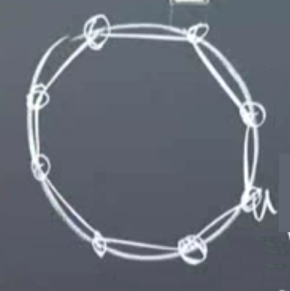
\includegraphics[width=10em]{compscieng_1_27_01.png}

Sınır şartımızı hatırlarsak düz cizgilerin çembere değdiği noktalarda $u = 0$.

$M$ tane köşe olsun, ve orta noktadan köşelere çizgiler çekerek üçgenler
oluşturalım, altta üçgenlerden biri görülüyor,

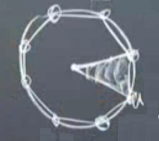
\includegraphics[width=10em]{compscieng_1_27_02.png}

Üçgenin alt iki köşesinde tabii ki $u = 0$ şartı geçerli. İki üçgen arasındaki
sınırda ise doğal sınır şartı denilen Neumann şartı geçerli olacak, eğimin
sıfır olma şartı, yani $\ud u / \ud n = 0$. Orijinde ne yapmam gerektiğinden
emin değilim şu anda. 

Gerçek bir problem işte burada. Muhakkak problem biraz yapay, çünkü analitik
çözümün ne olduğunu biliyoruz, ama mesela bu problemde hesap yapmak, hatanın
ne olacağını düşünmek, bunlar hala ilginç sorular ve ciddi işler. 

Bu problemi çözerken parçasal lineer öğeler (piecewise linear elements)
kullanmanızı isteyeceğim, daha önce bahsettiğim piramitler bunlar. Ama
bazılarınız karesel (quadratic) öğeler kullanmak isterse buna hayır demem.
Bu öğeler daha hassas / doğru sonuçlar verecektir. 

Şimdi ızgarayı daha detaylı şekilde yaratalım. Bir liste yaratacağız, bu listede
ızgara noktaları olacak, bu liste çözüm algoritmasina verilecek ve algoritma
oradan devam edecek.

Çember içinde daha önce yarattığımız üçgenlerden iki tanesini yanyana düşünelim,
en sağ üstteki nokta nerededir? $(\cos \pi/8, \sin \pi/8)$ değil mi? Sonra en
soldan en sağa $N$ tane (resimde $N=4$) düğüm daha koyarız, her aralık yatay
eksende $h$ büyüklüğünde olabilir, ve $N h = \cos\pi/8$ tabii ki. Sonra
dörtgenleri ortadan kesen çizgiler de ekliyorum ve alttaki şekil ortaya çıkıyor,

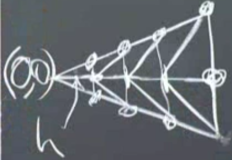
\includegraphics[width=15em]{compscieng_1_27_03.png}

Izgara düğüm noktalarına indis atamak iyi olur, soldan sağa önce orta çizgi
üzerinde 1,2,3,4,5 diye gideriz, sonra üst kenar, ardından alt, 13 tane düğüm
olur. Üçgenlere de indis atarız, 14 tane üçgen var. Düğüm noktalarının listesi
(0,0), (h,0), (2h,0), .. diye gidecek. Peki üçgenler? Onları köşe indisleriyle
belirtebiliriz, her üçgen için üç tane.

Bu listeleri alan kod bir $K$ matrisi oluşturur, matris eşsiz (singular) olur
çünkü sınır şartları daha içinde yok. En sağ üç nokta sıfırlandıktan sonra
(sınır şartı onları etkiliyor) matris tersi çevrilebilir hale gelir, ve $Ku = f$
çözülür. Kodun yaptığı $K$ ve $f$'yi oluşturmak.

Üçgen şekilleri hakkında; üçgenlerin açıları ufak olmayacak şekilde seçin dedik
fakat probleme göre bu değisebilir, mesela bir uçak kanadının aerodinamik
simülasyonu için FEM kullanıyorsanız, havanın akışı yönünde ince ince üçgenler
koymak gerekebilir çünkü ilginç olan fiziki fenomen o boyutta vuku bulmaktadır.

Şimdi bir adım geriye atıp resme bir daha bakalım. Matrisi oluştururken temel
aldığımız formül Poisson / Laplace denklemlerini zayıf formu. Güçlü formdan
başlayalım,

$$
-u_{xx} - u_{yy} = f(x,y)
$$

Zayıf forma geçmek için iki tarafı bir deneme fonksiyonu ile çarpıyorum,
ve tüm alan üzerinden entegralini alıyorum,

$$
\int \int (-u_{xx} - u_{yy}) v(x,y) \ud x \ud y =
\int \int f(x,y) v(x,y)  \ud x \ud y
$$

Üstteki ``tüm mümkün (admissable)'' $v(x,y)$'ler için yapılır. Ana fikir şu eğer
üstteki geniş bir $v$ ailesi için doğruysa bunun olmasının tek yolu sol tarafta
çarpılanların sağ tarafta çarpılanlara eşit olması, çıtlatılan temel yardımcı
önerim (lemma) bu.. Burada sözel olarak belirttik daha kuramsal şekilde de
ispatı var ama, ana fikir güçlü formun zayıf forma olan eşitliği.

Sonraki adım nedir? Eşitliğin sağ tarafı iyi ama sol taraf daha iyi olabilir,
sol tarafta ikinci türev var, ve benim piramid fonksiyonlarımın ikinci türevleri
yok. O zaman parçalı entegrasyon tekniğini uygularım, böylece türevi $u$'dan
$v$'ye geçirebilirim, böylece $u$'da tek türev kalır ve böylece piramitlerimi
kullanabilirim. 

Parçalı entegrasyon tekniğinin iki boyutlu versiyonunu kullanmam lazım. Green'in
formülü gerekli, ya da Gauss-Green formülü. 

$$
\int \int -\bdiv (\grad u) v \ud x \ud y
$$

ile başlıyoruz, $\bdiv$ $v$'ye gidince artı oluyor, devriği alınıyor $\grad$
oluyor, 

$$
= \int \int (\grad u) (\grad v) \ud x \ud y  +
\oint (\grad u \cdot n) v
$$

Ya da farklı bir formda şöyle yazabilirim, 

$$
\int \int
(
\frac{\ud u}{\ud x} \frac{\ud v}{\ud x} +
\frac{\ud u}{\ud y} \frac{\ud v}{\ud y} 
) =
\int \int f(x,y) v(x,y)  \ud x \ud y
$$



[devam edecek]

Kaynaklar

[1] {\em 18.085 SUMMER 2012 Site},
    \url{https://math.mit.edu/classes/18.085/2012summer.html}

\end{document}
